\documentclass[twoside,11pt]{article}

% Any additional packages needed should be included after jmlr2e.
% Note that jmlr2e.sty includes epsfig, amssymb, natbib and graphicx,
% and defines many common macros, such as 'proof' and 'example'.
%
% It also sets the bibliographystyle to plainnat; for more information on
% natbib citation styles, see the natbib documentation, a copy of which
% is archived at http://www.jmlr.org/format/natbib.pdf

\usepackage{jmlr2e}
\usepackage{graphicx}
\usepackage{xcolor} % for color names
\graphicspath{{./}}

% Definitions of handy macros can go here

\newcommand{\dataset}{{\cal D}}
\newcommand{\fracpartial}[2]{\frac{\partial #1}{\partial  #2}}
\newcommand{\code}[1]{\texttt{#1}}
\newcommand{\titleofpaper}{Conformer-RL}
% Heading arguments are {volume}{year}{pages}{date submitted}{date published}{paper id}{author-full-names}

% TODO: update heading
% \jmlrheading{volume}{year}{pages}{date submitted}{date published}{paper id}{Jiang et al.}

% Short headings should be running head and authors last names
\ShortHeadings{\titleofpaper}{Jiang et al.}
\firstpageno{1}


\newcount\comments  % 0 suppresses notes to ourselves in text
\comments=0  % TODO: change to 0 for final version
\newcommand{\genComment}[2]{\ifnum\comments=1{\color{#1}{\textsf{\footnotesize #2}}}\fi}

\newcommand{\ambuj}[1] {\genComment{red}{[AT: #1]}}
\newcommand{\tarun}[1] {\genComment{blue}{[TG: #1]}}
\newcommand{\ziping}[1]{\genComment{green}{[ZP:#1]}}
\newcommand{\josh}[1]{\genComment{purple}{[JK:#1]}}
\newcommand{\exequiel}[1]{\genComment{orange}{[EP:#1]}}
\newcommand{\paul}[1]{\genComment{brown}{[PZ:#1]}}
\newcommand{\runxuan}[1]{\genComment{pink}{[RJ:#1]}}

\begin{document}

\title{\titleofpaper: A Deep Reinforcement Learning Library for Conformer Generation}

\author{\name Runxuan Jiang$^1$ \email runxuanj@umich.edu \\
       \name Tarun Gogineni$^1$ \email tgog@umich.edu \\
       \name Joshua Kammeraad$^{2, 3}$ \email joshkamm@umich.edu\\
       \name  Yifei He$^1$ \email heyifei@umich.edu \\
       \name Ambuj Tewari$^{1, 2}$ \email tewaria@umich.edu\\
       \name Paul Zimmerman$^3$ \email paulzim@umich.edu\\
       \\
       \addr $^1$Department of EECS, University of Michigan, USA\\
       \addr $^2$Department of Statistics, University of Michigan, USA\\
       \addr $^3$Department of Chemistry, University of Michigan, USA
}

\editor{TBD}

\maketitle

%\newpage

\begin{abstract}%   <- trailing '%' for backward compatibility of .sty file
  We present \code{\titleofpaper}, an open-source deep reinforcement learning library for molecular conformer generation using Python. The library contains modular interfaces for environments and agents, allowing users to easily build and test new implementations. We also include several pre-built models and agents using state-of-the-art algorithms to serve as performance baselines. Additionally, \code{\titleofpaper} comes with extensive logging and visualization tools for evaluation of agents and generated conformers, as well as a toolkit for generating and modifying molecules. \code{\titleofpaper} is well-tested and thoroughly documented, and is available on PyPi and Github: \url{https://github.com/ZimmermanGroup/conformer-rl}.
\end{abstract}

\begin{keywords}
  deep reinforcement learning, graph neural network, open source, conformer generation, computational chemistry
\end{keywords}

% \ambuj{paper format roughly based on \href{https://www.jmlr.org/papers/volume22/20-376/20-376.pdf}{ChainerRL}. also used this one but it is less related: \href{https://www.jmlr.org/papers/volume22/20-451/20-451.pdf}{Python Optimal Transport}}

\section{Introduction}
Several recent works have applied deep reinforcement learning to tasks in computational chemistry \citep{li2018foldingzero,zhou2017reactions,simm2020moldesign}. One task where deep reinforcement learning has shown promising results is conformer generation \citep{gogineni2020torsionnet}, which involves finding an ensemble of unique low-energy three-dimensional orientations, or conformers, for a given molecule \citep{ebejer2020confgen}. Efficient and accurate prediction of low-energy conformers is integral to molecular modeling, with wide applications from drug development to 3D QSAR \citep{cole2018confgen}. Thus, there is a need for a modular and extensible open-source software library for deep reinforcement learning applied to conformer generation.
% \tarun{we should cite an example of one that does exist with these shortcomings} \runxuan{I think I mention a few specific shortcomings of existing papers/code in the next two paragraphs. Also there isn't a lot of papers specifically about conformer generation, but there are several about using RL with protein folding, so perhaps I can include an example of that.}
In this paper, we introduce \code{\titleofpaper}, a comprehensive and modular Python library for applying deep reinforcement learning to conformer generation, using PyTorch \citep{torch} for deep learning and RDKit \citep{Landrum2016rdkit} for chemoinformatic capabilities.

Many libraries already exist that contain benchmarking experiments for general deep reinforcement learning. For example, OpenAI Gym \citep{brockman2016gym} and bsuite \citep{osband2020bsuite} both contain implementations of reinforcement learning environments used for benchmarking agents. \code{\titleofpaper} seeks to fill this role within the conformer generation space by supplying pre-built environments for benchmarking on this task. Additionally, \code{\titleofpaper} includes an interface to easily customize environments for further exploration within conformer generation and for custom tasks like reaction prediction.

There are also many implementations of baseline deep reinforcement learning agents available, such as RLlib \citep{liang2018rllib}. However, since the feature rich graphical representation of molecules is often unsupported out of the box in fixed-vector-state-based libraries, a large amount of modification and setup work is required to adapt these baseline libraries to work with molecular environments. Within \code{\titleofpaper}, we include a general agent base class for building agents compatible with conformer generation environments, as well as several baseline reinforcement learning algorithms.

Finally, \code{\titleofpaper} provides analysis and logging modules for recording and visualizing training results, including conformer-generation specific metrics and visuals.

\begin{figure}[h]
  \centering
  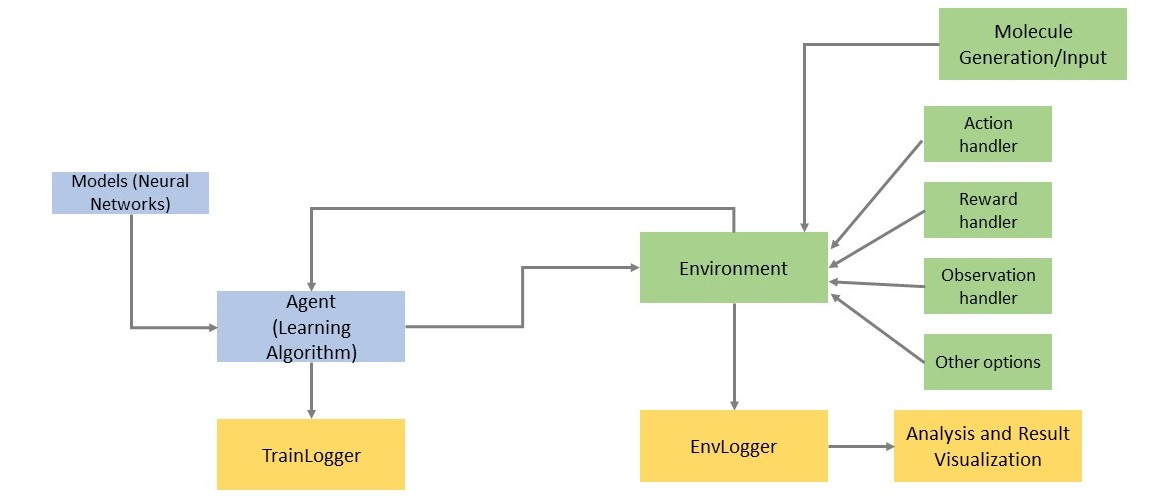
\includegraphics[width=\textwidth]{architectures.jpg}
  \caption{Architecture of \code{\titleofpaper}. 
  % \paul{Conceptually, I'd think the horizontal axis should be flipped (ie most green boxs on the left, though environment centered would be nice). Rearrange the boxes so they flow in a more ordered way. Also, add legend with the color labels.}
  }
  \label{fig:architecture}
\end{figure}

\section{\titleofpaper \space Architecture}
  A visual representation of the architecture of \code{\titleofpaper} can be seen in Figure \ref{fig:architecture}.
  % \tarun{overall thoughts: we should describe more of the specific utils and conformer generation conveniences that we created, such as the molecule observation environments, or the reward counting via built in conformer rejection. As it stands most of the components we discuss here are not unique to our library.} \runxuan{I added a few sentences about specific examples of the environment handlers that are unique to our implementation. I think another option is to include an explicit list of the options available for each environment component but I think this is already covered by the API reference.} 


\subsection{Environments}
\code{\titleofpaper} environments are built on top of the \code{ConformerEnv} base class. Methods in \code{ConformerEnv} correspond to different components within the environment, each of which are independent to the behavior of other components. The main components include:
\begin{itemize}
  \item \textbf{Action Handler} determines how the molecule or molecule structure is modified given an incoming action. \code{\titleofpaper} provides action handlers for setting molecule conformation torsion angles for both discrete and continuous action spaces.
  
  \item \textbf{Reward Handler} returns a scalar reward based on the current configuration of the molecule. \code{\titleofpaper} includes several reward implementations derived from the energy of the current molecule conformoration, such as (but not limited to):
  \begin{itemize}
    \item \textbf{Basic Energy Reward} - basic reward that is inversely correlated with the energy of the current conformer.
    \item \textbf{Pruning Energy Reward} - reward that ``prunes" (returns a 0 reward) any conformer generated from an action already seen in the current episode.
    \item \textbf{Gibbs Score Reward} - the reward used in \citet{gogineni2020torsionnet}, which prunes conformers based on a TFD (torsional fingerprint deviation) derived metric.
  \end{itemize}

  \item \textbf{Observation Handler} returns a graph representation for the current molecule conformation. \code{\titleofpaper} contains several methods for extracting features from molecules and converting a conformation into a PyTorch Geometric graph structure, such as:
  \begin{itemize}
    \item \textbf{Node Feature Extractors} - extracts information about atoms in a molecule which can be included in the nodes of the graph representation, such as atom element and three-dimensional coordinates.
    \item \textbf{Edge Feature Extractors} - extracts information from molecules that can be represented as edges in the graph reperesentation, with options for including bonds between atoms, bond type, Euclidean distances, and more.
    \item \textbf{Graph Normalizers} - normalizes the graph representation of molecules in terms of translation, rotation, and/or scale.
  \end{itemize}

  % \tarun{should we describe also the normalizations and extra edges we add by preprocessing or would that be out of the scope}
\end{itemize}
Other class methods of \code{ConformerEnv} can also be overridden at the user's convenience. For example, if the user would like to keep track of the number of conformers generated with an energy below a certain threshold for each episode, they may add a member variable \code{self.confs\_below\_threshold = 0} to the \code{reset()} method, and then update \code{self.confs\_below\_threshold} within the action handler.

Due to the flexibility of the design of \code{ConformerEnv}, different handlers can be mixed and matched to form unique environments, and new environments for tasks related to conformer generation, such as protein folding and chemical reaction optimization, can be easily built by implementing custom variations of the components.

\code{\titleofpaper} also includes wrappers for executing multiple environments in parallel. 

  \subsubsection{Molecule Generation}
  \code{\titleofpaper} environments are designed to be configurable with different molecules, including user-generated ones. The molecular structure is specified as an RDKit molecule object. As a mature cheminformatics library, RDKit offers a standard means of representing and manipulating molecules and can directly interface files from a number of computational chemistry packages including MOL files. RDKit is also at the core of a broad ecosystem of other cheminformatics packages, including Open Babel, which has extensive conversion capabilities for over 100 formats \citep{Oboyle2011openbabel}. 
  
  Environments are initialized with a \code{MolConfig} object, which specifies the RDKit molecule to be used in the environment and any molecule-specific parameters. For convenience, \code{\titleofpaper} contains scripts for generating \code{MolConfig} objects for several simple molecules and molecule benchmarks found in \citet{gogineni2020torsionnet}, such as branched alkanes, lignin, and more. Molecule generation scripts utilize several libraries depending on the molecule, including stk \citep{Turcani2021stk}, stko \citep{Tarzia2021stko} and Lignin-KMC \citep{Orella2019ligninkmc}, with options for varying molecule size and structure. The currently available conformer generating tools were developed under the assumption of independently varying torsions. This model is sufficient for linear and branched molecules as well as molecules with rigid ring structures. Support for flexible ring structures, in which ring torsions may not vary independently, would be a valuable future contribution.
  
  % \josh{Citations for dependencies: is the install\_requires in setup.py the full list of direct dependencies? Could be good to look through and check that we aren't missing important ones to cite if we haven't already. I was thinking it'd be good to include citations for stk and stko especially since the authors have been responsive and helpful, and this seems like a good place. \url{https://github.com/lukasturcani/stk}, \url{https://aip.scitation.org/doi/10.1063/5.0049708}. stko doesn't have a paper but we can cite the GitHub: \url{https://github.com/JelfsMaterialsGroup/stko}}.

\subsection{Agents and Models}
Agents in \code{\titleofpaper} inherit from the \code{BaseAgent} class. Each agent is initialized with a \code{Config} object, which specifies the neural network model to be used, training environment, optimizer function, and other hyperparameters. Custom agents can be created by overriding the \code{step()} method of \code{BaseAgent}, which corresponds to one iteration of interacting with the environment to collect samples and then training on those samples.

\code{\titleofpaper} implements several agents using state of the art algorithms, including advantage actor critic (A2C) \citep{wu2017a2c} and proximal policy optimization (PPO) \citep{schulman2017ppo}. The software also includes baseline implementations of several neural network architectures compatible with molecular inputs, including versions of the model from \citep{gogineni2020torsionnet}. The networks are built using graph neural network components using PyTorch Geometric \citep{fey2019geometric} and are compatible with molecules of variable size.

\subsection{Logging and Analysis}
The \code{\titleofpaper} library contains two types of loggers. \code{TrainLogger} logs information from the agent during training, such as total reward per episode, training loss, runtime, etc., and supports logging data directly to TensorBoard \citep{tensorflow2015-whitepaper}, where the data can be visualized in real time. \code{EnvLogger} records environment information across a single environment interaction/episode, such as the conformers generated and conformer energies. \code{EnvLogger} supports saving the per-episode data and each generated molecule conformer as a MOL file. Both loggers are integrated into the \code{BaseAgent} and \code{ConformerEnv} interfaces, and are readily accessible when writing new agents or environments.

\begin{figure}[h]
  \centering
  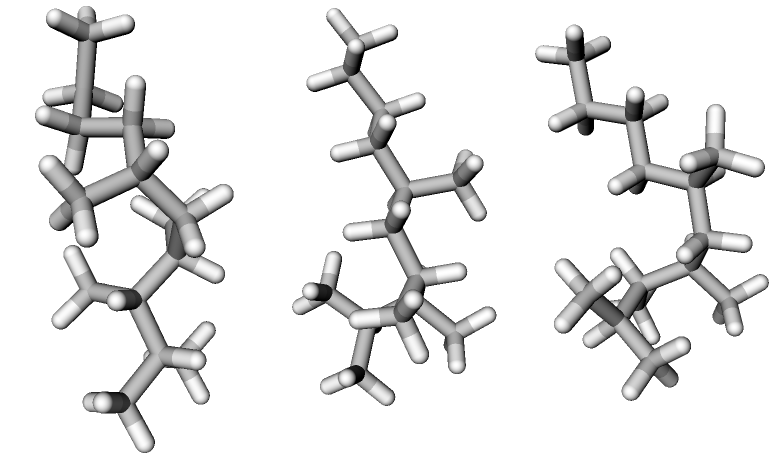
\includegraphics[scale=0.75]{molecules.png}
  \caption{
    Example of using the toolkit to visualize a generated conformer in Jupyter.
  }
  \label{fig:molecules}
\end{figure}

\code{\titleofpaper} contains an analysis toolkit for calculating and visualizing results. The toolkit is designed to be used in a notebook and provides convenience methods for generating figures, charts, and interactive 3D visuals for molecule conformers (Figure \ref{fig:molecules}).

\section{Conclusion}
\code{\titleofpaper} is a comprehensive library for training and testing deep reinforcement learning agents in the conformer generation task. \code{\titleofpaper}'s modular interfaces can increase research reproducibility and stimulate discovery in conformer generation. Full documentation can be found at \url{https://conformer-rl.readthedocs.io/en/latest/}.



\newpage
% Acknowledgements should go at the end, before appendices and references

\acks{
  We acknowledge the support of NSF via grants DMS-1646108,  IIS-2007055, and CHE-1551994.
}

\vskip 0.2in
\bibliography{reference}


% Manual newpage inserted to improve layout of sample file - not
% needed in general before appendices/bibliography.

\newpage

% \appendix
% \section*{Appendix A.}

\end{document}